\chapter{Scale Space} \label{chap:scale-space}

One of the fundamental challenges in building systems that can understand images is the construction of good \textit{representations}.  Since even a relatively small image comprises a vast quantity of data, we would like to distill the information down to a much more compact form that tells us about the things we care about in the image and is \textit{invariant} to things we don't care about.  

Early work focused on simple representations of an image, such as the extrema in the signal (e.g. edges, dots etc.) and their first or second derivatives - a line sketch can contain much of the semantic content of an image while requiring far fewer bits of information to store.  However, this approach quickly runs into difficulties.  Over what scale should the derivatives of the image signal be taken?  Edges which define important for objects at one scale, such as the grains on a piece of wood, are irrelevant at another scale, such as a picture of a forrest. 

There have been several major contributions in this area, but perhaps the most important was the introduction of \textit{scale space filtering} \cite{witkin1987scale}.  The core idea is that the image should be represented simultaneously by a set of multiple scales.  This is achieved by simply convolving the source image with Gaussian filters of increasing bandwidth (this is illustrated with a one dimensional signal in Fig.~\ref{fig:scales}).  

\begin{figure}
\centering
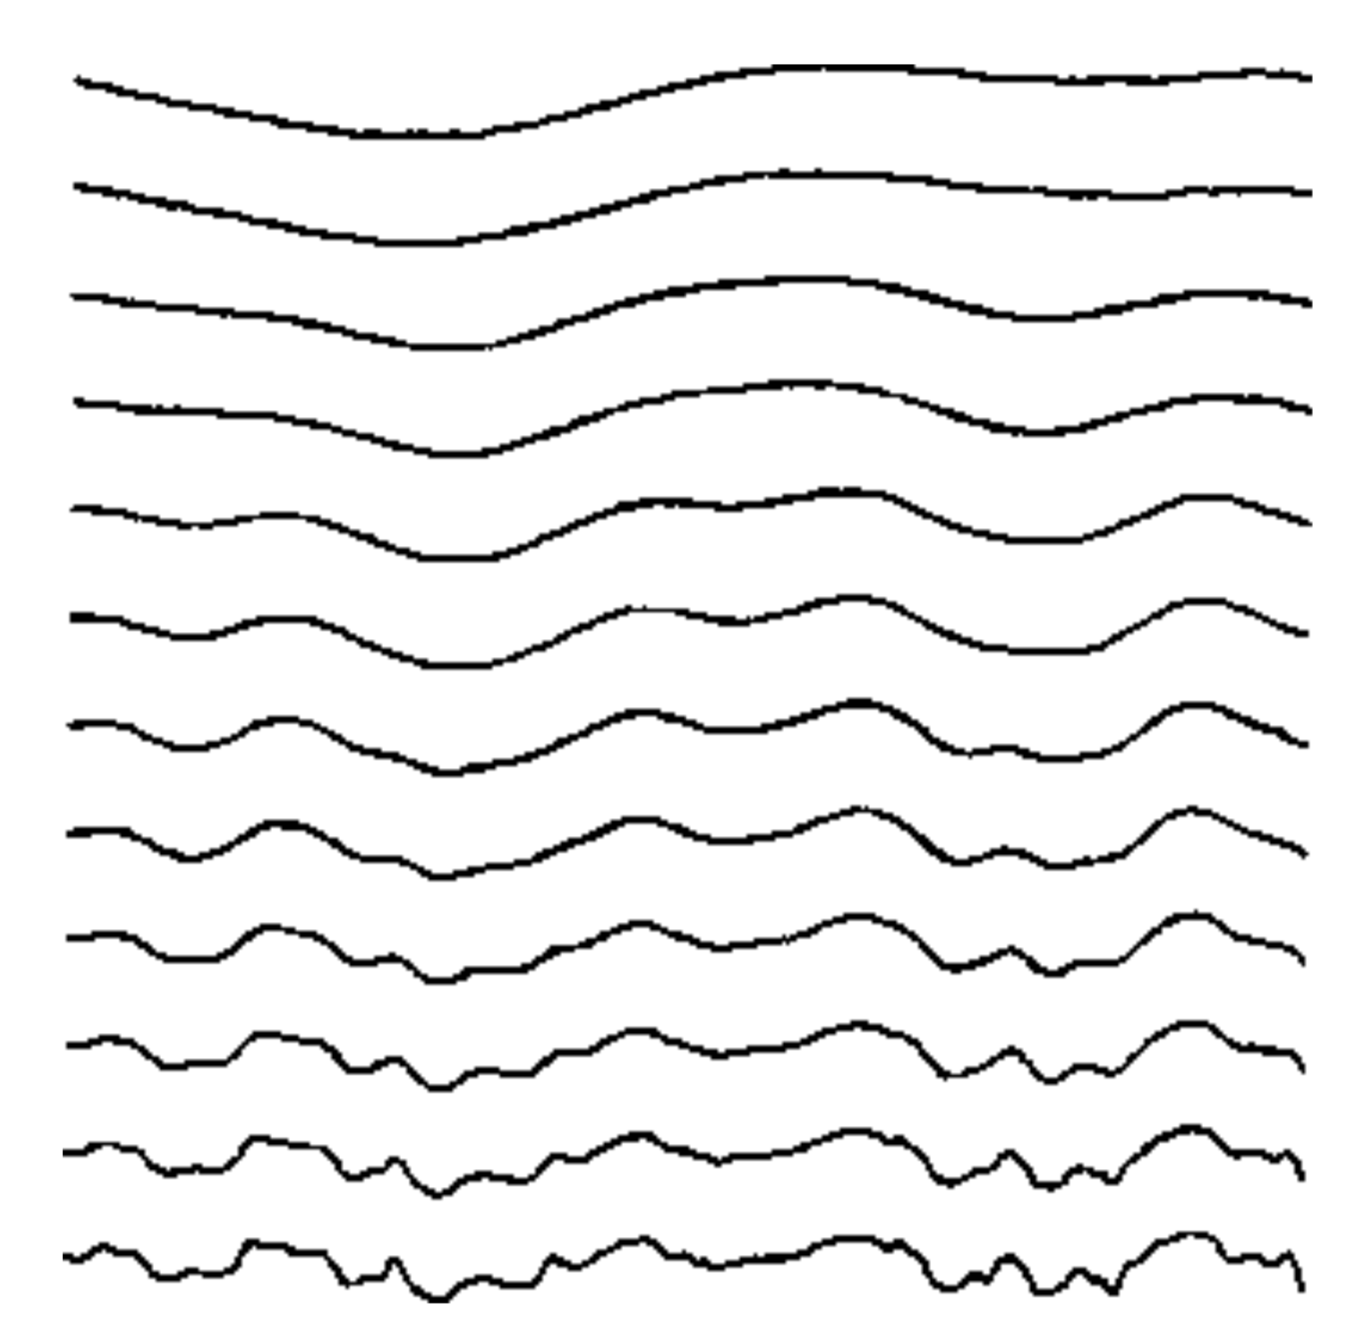
\includegraphics[height=0.3\textwidth]{figs/scale-space.png}
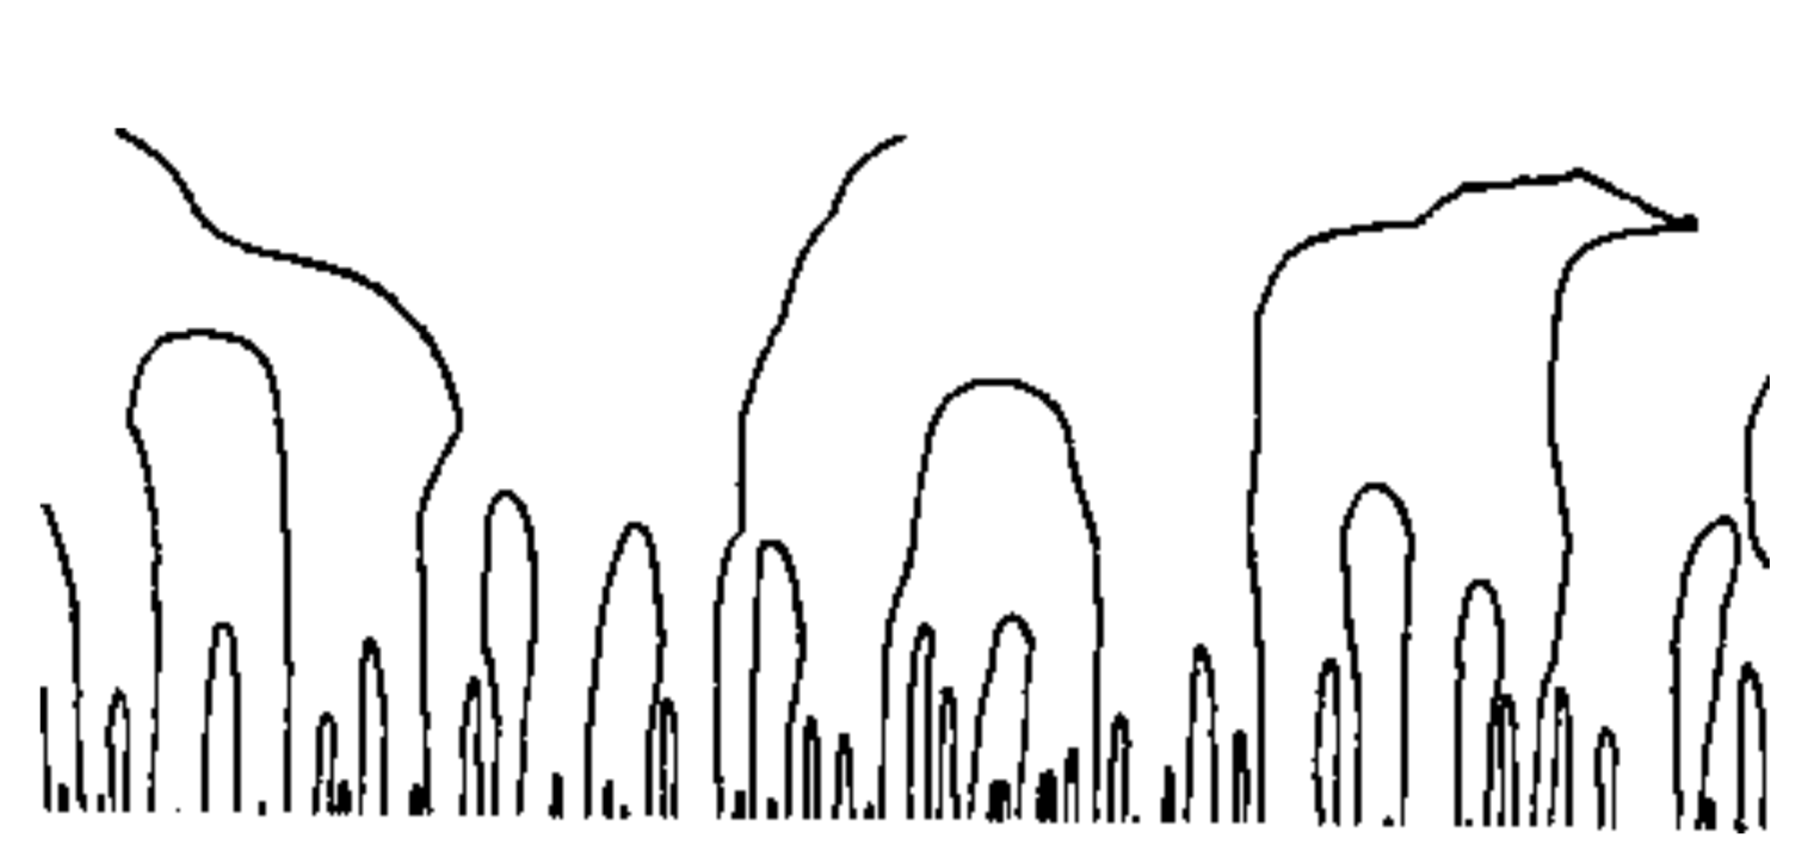
\includegraphics[height=0.25\textwidth]{figs/zero-crossings.png}
\caption{\textbf{Left}: The scale space of a one-dimensional signal $\phi$.  At the bottom is the raw signal, which has been smoothed by Gaussian kernels with increasing bandwidth as you move up the figure. \textbf{Right:} The level sets $ \phi_{xx} = $ corresponding to the scale space shown on the left.  In both images the $x$-axis is horizontal and the vertical axis represents the value fo $\sigma$ (the bandwidth of the smoothing kernel). These figures originally appeared in \cite{witkin1987scale}).\label{fig:scales}}
\end{figure}

In the original work, Witkin focused on using the zeros of the second derivative (i.e. the inflection points) of the signal as the representation